%!TEX root = ../../../report.tex
\section{The study of bipedalism}
\label{sec:bipedalism}

The current human bipedal locomotion arises from the combination of a big variety of subsystems working in conjunction to achieve the intended gait generation according to the requirements of the situation.
The biomechanics of the limbs, consisting in bones, muscles and tendons under the control of the nervous system yields the adequate production of the different motion patterns in order to displace the body as energetically efficiently as possible.
This complex behavior is the result of 4 million years of an evolution \cite{bipedalism2} that started in primates and that has entailed both morphological and neurological changes in the human body since the first bipedal hominids to the current structure in Homo sapiens.
There exist several different theories about the reasons that originated and led to the adaption of this posture and bipedal motion.
Although different, most of them assume that most of them assume that the development of this structural and behavioral changes arose from a change in the environment in pre-hominids, for with bipedal behavior suddenly offered some kind of survival value \cite{bipedalism1}.
However, the genus Homo is not the only species that has evolved towards two-legged locomotion
Currently there are a few more species that have reached this method of displacement as a result of a natural selection process in which bipedalism offered the broadest set of advantages of the specie being the main ones listed below. 

\begin{itemize}
	\item Erect posture for a wider field of view and reach range.
	\item Free forelimbs, that could evolve towards specialized, non-locomotory applications such as object manipulation, combat, flight, etc.
	\item Faster displacement in certain species, although not generally.
\end{itemize}

Extensive research in the actuation and control structures involved in human bipedalism has been conducted from within the scientific fields of anthropology, biology, medicine, sport science and lately, several areas withing the engineering.
Its goal, as per definition of science, has been to reach a full understanding of what led to this behavior and the knowledge of how it functions, together with the discovery of ways in which it can be mimicked and improved, aiming at a more inexpensive and optimized locomotion.
This last fact has led to the belief that the next stage in the evolution of human locomotion will not come from nature as until nowadays, but from the hand of science and engineering, which has been lately depicted in literature and pop-culture as in \ref{fig:biped_evolution}.

\begin{figure}[h]
	\centering
	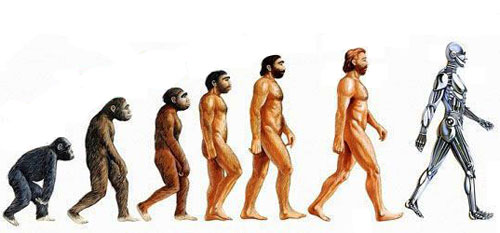
\includegraphics[width=0.8\textwidth]{figures/artificialhumans.jpg}
	\caption{Evolution of bipedalism (artistic depiction from \cite{human_evol_fig})}
	\label{fig:biped_evolution}
\end{figure}

\subsection{Bipedalism and engineering} % (fold)
\label{sub:bipedalism_and_engineering}
The discipline of engineering has been historically among the latest of the cited ones to start its contribution to the research and improvement of biped motion in a well defined manner, although its earliest contributions seem to date from ancient Egypt and Hinduism 
From the study of human bipedal motion described above, the insights emerged on its functioning together with the need to repair, improve or imitate its functionality led to the creation of new branches within the discipline of engineering.
The three most relevant ones for the present thesis are listed and introduced below.

\begin{enumerate}
	\item Prosthetics
	\item Orthotics
	\item Humanoid robots  **(find better name)
\end{enumerate}


\paragraph{Prosthetics} % (fold)
\label{par:prosthetics}

% paragraph prosthetics (end)

\paragraph{Orthotics} % (fold)
\label{par:orthotics}

% paragraph orthotics (end)

\paragraph{Humanoid robots} % (fold)
\label{par:humanoid_robots}

% paragraph humanoid_robots (end)

\begin{figure}[h]
	\centering
    \begin{subfigure}[b]{0.3\textwidth}
        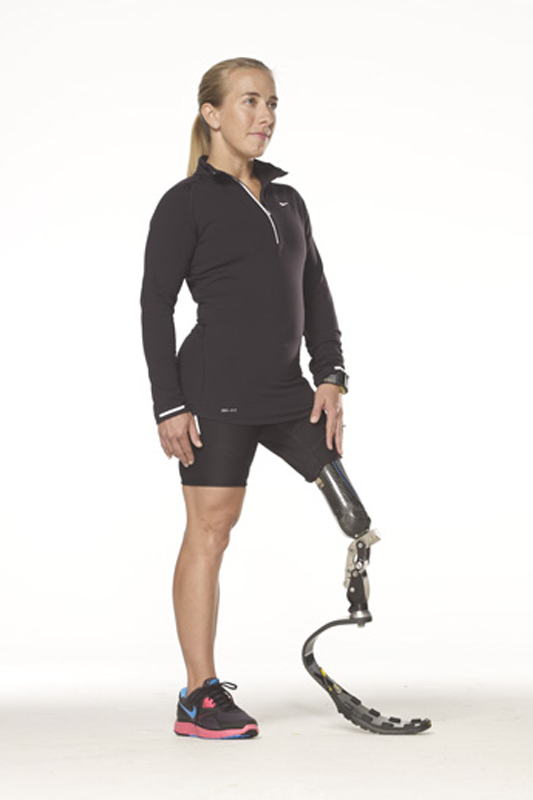
\includegraphics[width=\textwidth]{figures/prosthetic_leg.png}
        \caption{Prosthetic leg, Colorado Springs Co.}
        \label{fig:prosthetic_leg}
    \end{subfigure}
    \centering
    \begin{subfigure}[b]{0.3\textwidth}
        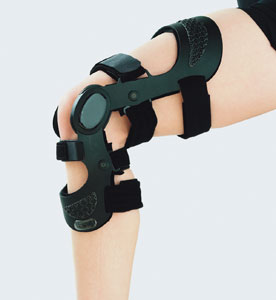
\includegraphics[width=\textwidth]{figures/orthotic_leg.jpg}
        \caption{Knee brace, New Hope Co. model}
        \label{fig:orthotic_leg}
    \end{subfigure}
    \centering
    \begin{subfigure}[b]{0.3\textwidth}
        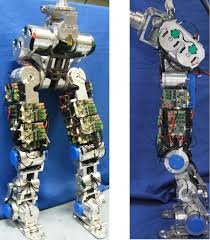
\includegraphics[width=\textwidth]{figures/robotic_leg.jpg}
        \caption{Robotic legs, COMAN robot \cite{coman}}
        \label{fig:robotic_leg}
    \end{subfigure}
\end{figure}
\todo{Rearrange/find other figures}


% subsection bipedalism_and_engineering (end)

